hfill На правах рукописи

\vspace{\baselineskip}
\vspace{\baselineskip}
\vspace{\baselineskip}
\vspace{\baselineskip}

\noindent\centerline{\bf{Никифоров Александр Александрович}}

\vspace{\baselineskip}
\vspace{\baselineskip}
\vspace{\baselineskip}
\vspace{\baselineskip}

\noindent\centerline{РАЗРАБОТКА АЛГОРИТМА ДЕТЕКТИРОВАНИЯ}
\noindent\centerline{СИГНАЛОВ В СИСТЕМАХ С КОДОВЫМ РАЗДЕЛЕНИЕМ КАНАЛОВ}

\vspace{\baselineskip}
\vspace{\baselineskip}
\vspace{\baselineskip}
\vspace{\baselineskip}

\noindent\centerline{Специальность 05.13.01. – Системный анализ, управление и обработка информации}

\vspace{\baselineskip}
\vspace{\baselineskip}
\vspace{\baselineskip}
\vspace{\baselineskip}

\noindent\centerline{Автореферат} 
\noindent\centerline{диссертации на соискание ученой степени}
\noindent\centerline{кандидата технических наук}


\vspace{\baselineskip}
\vspace{\baselineskip}
\vspace{\baselineskip}
\vspace{\baselineskip}
\noindent\centerline{\bf{ЧЕРНОВИК}}

\vfill
\noindent\centerline{Москва – 2013}

\pagenumbering{gobble}
\newpage
%%%%%%%%%%%%%%%%%%

\noindent{Работа выполнена в Московском Государственном Университете Приборостроения и Информатики}
\vspace{\baselineskip}
\vspace{\baselineskip}
\vspace{\baselineskip}
\vspace{\baselineskip}

\noindent
\begin{tabular}{ l r }
Научный руководитель -	& 	Мацнев Анатолий Петрович \\
		 	&	Профессор, кандидат технических наук \\
\end{tabular}

\vspace{\baselineskip}
\vspace{\baselineskip}
\vspace{\baselineskip}

\noindent
\begin{tabular}{ l r }
Официальные оппоненты: 	& 	 \\
		 	&	 \\
\end{tabular}

\vspace{\baselineskip}
\vspace{\baselineskip}
\vspace{\baselineskip}

\noindent
\begin{tabular}{ l r }
Ведущая организация: & Название
\end{tabular}

\vspace{\baselineskip}
\vspace{\baselineskip}
\vspace{\baselineskip}

\noindent
Защита состоится Дата 

\vspace{\baselineskip}
\vspace{\baselineskip}
\vspace{\baselineskip}

\noindent
на заседании диссертационного совета XXX при 

\vspace{\baselineskip}
\vspace{\baselineskip}
\vspace{\baselineskip}

\noindent
С диссертацией можно ознакомиться в библиотеке 

\noindent
Автореферат разослан  11 сентября 2009 г.

\vfill
\noindent
Учёный секретарь диссертационного совета\hfill Фамилия

\pagenumbering{gobble}
\newpage

% switch page on
\pagenumbering{arabic}

%\addcontentsline{toc}{section}{ВВЕДЕНИЕ}
\section*{Общая характеристика работы}

\paragraph{Актуальность работы}. Диссертация посвящена разработке алгоритма детектирования сигнала и оценки частоты
в системах с расширенным спектром.
)
Большое количество современных систем являются беспроводными. Простота развертывания, мобильность, относительно низкая
стоимость - вот основные преимущества беспроводных систем. Количество мобильных устройств (телефоны, планшетные компьютеры
и т.д.) с каждым годом стремительно растет, только мобильных телефонов в 2011 году было 5.6 миллиарда и покрывало 79.86\%
 населения земли. Технологии беспроводной связи глубоко проникли во все сферы жизни общества:
обеспечение безопасности с помощью RFID датчиков, предоставление доступа в интернет по техноолгиям 3G, WiFi, 
сотовая связь по различным технологиям (GSM, CDMA, DAMPS). Некоторые из этих систем строятся на основе методики
расширения спектра, которая отвечает современным требованиям по мощности сигнала, а так же по безопасности передаваемых
данных. В основе таких систем лежат шумоподобные (широкополосные) сигналы (ШПС). Вместе с тем растут требования к таким
системам. Применение ШПС ставит ряд специфических задач по обработке информации, обусловленных особенностями ШПС.
Свойства характерные для ШПС, выгодно отличают данный класс систем от класса узкополосных систем, но с другой стороны
оборачивается усложнением методов обработки ШПС. В России в этой области занимались В.Б. Пестряков, Л.Е. Варакин, В.Е. Гантмахер и др.

В конце 40-х-начале 50-х годов прошлого века Мортимер Рогофф провёл эксперимент по передаче информации при помощи
псевдошумового сигнала. За последующие полвека сложность систем и производительность электронной техники многократно
выросли. В то же время распространение беспроводных устройств возрастает, что требует разработки новых более
эффективных алгоритмов обработки сигналов. Особенностью систем с расширенным спектром является, то что после повторной
модуляции псевдослучайной последовательностью (ПСП) в сигнале присутствует одна гармоническая компонента.
Это позволяет эффективно использовать параметрические методы
оценки частоты сигнала. Однако, отсношение сигнал / шум (ОСШ) входного сигнала не всегда достаточно для получения требуемой точности оценки.

При решении задач реализации и разработки алгоритмов обработки сигналов следует учитывать современную тенденцию - разработку
программных приемников. Данный подход обладает огромным преимущетвом - низкая стоимость разработки и тестирования. В то же
время производительность программных приемников не может сравниться с производительностью специализированных приемовычислителей.

В данной работе развивается подход к оценке частоты широкополосного сигнала на основе параметрического метода. Для проверки
теоретических результатов была реализована модель канала данных с использованием математического пакета Matlab. Были получены
рабочие характеристики предлагаемых алгоритмов и проверены 

\paragraph{Целью данной работы} являлась разработка и исследование алгоритмов на основе параметрического метода оценки частоты в системах 
с расширенным спектром, а так же сравнение развиваемого и традиционного подходов.

\paragraph{Научная новизна работы}
\begin{enumerate}
	\item{Предложено использовать параметрический метод оценки спектра для оценки частоты сигнала в системах с расширенным спектром.}
	\item{Предложен способ подавления окрашенного шума на основе итеративного вычисления автокорреляционной функции для
		получения несмещенной оценки частоты с использованием параметрического метода оценки спектра.}
	\item{Предложен способ вычисления автокорреляционной функции на основе быстрого преобразования Фурье.}
	\item{Предложен способ комбинации результата работа алгоритма оценки фазы ПСП Delay And Multiply Approach, алгоритма итеративной оценки АКФ и
		параметрического метода оценки спектра в задаче детектирования и оценки сигнала с расширенным спектром.}
\end{enumerate}

\paragraph{Научная и практическая значимость работы}
\begin{enumerate}
	\item Предложен алгоритм детектирования сигнала с расширенным спектром на основе параметрического метода с существенным
		сокращением вычислительных затрат в сравнении с традиционным методом для одного источника.
	\item Предложен способ оптимизации вычисления АКФ, что позволяет применять его в приемниках в режиме реального времени.
	\item Предложен алгоритм детектирования сигнала с расширенным спектром на основе параметрического метода и алгоритма DMA,
		что позволило свести перебор в двух областях: фаза ПСП и частота к перебору только в области фазы ПСП. Уточненное
		значение АКФ вычисляется с помощью предложенного в данной работе усовершенствованного итеративного алгоритма вычисления
		АКФ. Оценка частоты производится с помощью авторегрессионной модели.
	\item {Подход, предложенный в работе, позволяет произвести оценку частоты на ограниченном отрезке сигнала, без накопления;}
	\item{Проведен анализ вычислительных затрат развиваемого и классического подходов.}
\end{enumerate}

\paragraph{Основные научные положения, выносимые на защиту}
\begin{enumerate}
	\item {Алгоритм итеративного вычисления автокореляционной функции может быть эффективно реализован с исппользованием быстрого преобразования Фурье.}
	\item {Окрашенный шум может быть эффективно подавлен при помощи алгоритма итеративного вычисления автокореляционной функции.}
	\item {Параметрический метод оценки спектра может быть использован для детектирования и оценки частоты широкополосного сигнала.}
\end{enumerate}

\paragraph{Методы исследований.} Задачи исследования решаются при помощи методов теории сигналов, теории автоматического управления,
методов параметрического спектрального анализа, методов математического и имитационного моделирования.

\paragraph{Достоверность научных положений, результатов и выводов}

\paragraph{Апробация работы}
Основные научные результаты, полученные в ходу работы докладывались и обсуждались на:

Международной конференции "Радиоэлектронные устройства и системы для инфокоммуникационных технологий - РЕС-2013"

\paragraph{Публикации}
\begin{enumerate}
	\item Никифоров А.А., "ОПТИМИЗАЦИЯ АЛГОРИТМА ПОСЛЕДОВАТЕЛЬНОГО ВЫЧИСЛЕНИЯ АВТОКОРРЕЛЯЦИОННОЙ ФУНКЦИИ".
		Образование. Наука. Научные кадры., №5, 2013 (в публикации)
	\item Никифоров А.А.,"АЛГОРИТМ ИТЕРАТИВНОГО ВЫЧИСЛЕНИЯ АВТОКОРРЕЛЯЦИОННОЙ ФУНКЦИИ В ЗАДАЧЕ ОЦЕНКЕ ЧАСТОТЫ ШИРОКОПОЛОСНОГО СИГНАЛА".
		Механизация строительства, Ноябрь, 2013 (в публикации)
	\item Никифоров А.А. Мельников А.О. Токарев С.В. "Детектирование сигналов с расширенным спектром на основе АР модели, Промышленные АСУ и контроллеры", Май 2013, стр. 51-54.
	\item Никифоров А.А. "ДЕТЕКТИРОВАНИЕ СИГНАЛОВ С РАСШИРЕННЫМ СПЕКТРОМ НА ОСНОВЕ АР МОДЕЛИ С УЧЕТОМ МОЩНОСТИ ШУМА", Международная конференция
		"Радиоэлектронные устройства и системы для инфокоммуникационных технологий - РЕС-2013", Москва, Россия, доклады. Выпуск LXVIII. стр. 139.
	\item Никифоров А.А., Мельников А.О. "Методы детектирования систем спутниковой навигации". Интеллектуальный потенциал XXI века: ступени познания:
		Сборник мат-в V Международной студенческой научно-практической конференции: в 2-х частях. Часть 2 / Под общ. Ред. С.С.Чернова. – Новосибирск:
		Издательство НГТУ, 2011. – СС. 66 - 70. – 0, 2 п.л.
\end{enumerate}

\paragraph{Личный вклад автора.}
В основу диссертации легли результаты исследований, выполненных лично автором на кафедре «Управление и моделирование систем» Московского Государственного
Университета Приборостроения и Информатики. Личный вклад автора состоял также в непосредственном участии в получении исходных данных, в апробации результатов исследования,
в подготовке основных публикаций по выполненной работе.

\paragraph{Объём и структура диссертации}
Диссертация состоит из введения, четырех глав, заключения и списка литературы.

\section*{СОДЕРЖАНИЕ РАБОТЫ}

% Include text from phd
В первой главе рассматривается сигнал с расширенным спектром полученный методом "прямой последовательности".
Данный метод заключается в том, что гармоническая несущая сигнала модулируется высокоскоростным (широкополосным)
расширяющим сигналом \cite{sklyar}. Методы генерации таких последовательностей рассмотрены, например, в \cite{gantmaher-book, varakin-book, pestryakov-book}.
В данной работе в качестве ПСП используется код Голда. Свойства данного семейства ПСП подробно рассмотрены в \cite{gold-ieee},
а так же краткое описание свойств без доказательства приведены в \cite{tsui, akos-book}. Метод генерирования ПСП подробно рассмотрен
во многих источниках \cite{tsui, akos-book, kaplan} и в данной работе рассматриваться не будет.

В данном типе модуляции информационные сообщения кодируются изменением фазы несущей сигнала.
Математическую модель сигнала спутниковой системы навигации (СНС) Navstar GPS можно представить формулой \cite{tsui, akos-book, kaplan}:

\begin{equation}
	\label{eq:cdma_eq}
	s_k(t)=D_k(t)C_k(t)\cos{(\omega_{k}t + \phi_k(t))} + n_k(t)
\end{equation}
где ${D_k}$- информационный бит, ${C_k}$ - расширяющий код, ${\phi_k(t)}$ - фаза обусловленная допплеровским смещением частоты, а так же шумом осциллятора
и ${n_k(t)}$ - шумовая компонента. Формула  \ref{eq:cdma_eq} представляет математическую модель сигнала для спутника номер ${k}$.
Всего в группировке спутников Navstar GPS доступно 32 спутника. После повторного модулирования сигнала, указанного в выражении \ref{eq:cdma_eq},
получается:

\begin{equation}
	\label{eq:cdma_strip_eq}
	x_k(m)=\cos{(\omega_{k}m + \phi_k(m))} + n_k(m)
\end{equation}
Информационный бит принят за константу, так как в случае смены бита гармонический характер сигнала нарушается и детектирование становится невозможным.

\paragraph{Вторая глава} содержит разделы о параметрическом спектральном оценивании и автокоррелляционном анализа в приложении к детектированию и оценке
частоты сигнала в широкополосных системах.

\paragraph{Третья глава} состоит из предлагаемого усовершенствованного алгорита оценки автокореляционной функции (АКФ) с использованием
быстрого преобразования Фурье, алгоритма оценки частоты широкополосного сигнала на основе АР модели,
развиваемого подхода оценки параметров широкополосного сигнала 
при помощи комбинации алгоритмов Delay and Multiply Approach для оценки фазы ПСП, компенсации 
окрашенного шума на основе усовершенствованного алгоритма оценки АКФ и параметрического метода оценки спектра
для оценки параметров широкополосного сигнала.

Точность АР метода напрямую зависит от точности оценки АКФ гармонического сигнала.
Существует несколько способов компенсации шума для АР анализа.
Основным способом повышения точности оценки АКФ является увеличение размера выборки, что в случае модулированного сигнала может быть затруднительным. 

В данной работе предлагается использовать алгоритм увеличения ОСШ методом последовательного вычисления АКФ.
Для снижения вычислительных затрат последовательное вычисление АКФ предлагается реализовывать с использованием процедуры БПФ. 

Уточненная оценка АКФ на ${K}$-ом шаге данного алгоритма может быть получена с помощью выражения:
\begin{center}
\begin{equation}
	\label{eq:akf_3}
	\hat{r}_K = F^{-1}\left[ \left| Fx \right| ^{2^K} \right],
\end{equation}
\end{center}
где ${x}$ – вектор входного сигнала после снятия ПСП, ${F}$ – матрица прямого преобразования Фурье,
${F^{-1}}$ - матрица обратного преобразования Фурье.

Схематически алгоритм получения уточненной оценки АКФ на третьем шаге представлен на рисунке \ref{pic:akf_pic}.
\begin{figure}[H]
	\center\scalebox{0.8}{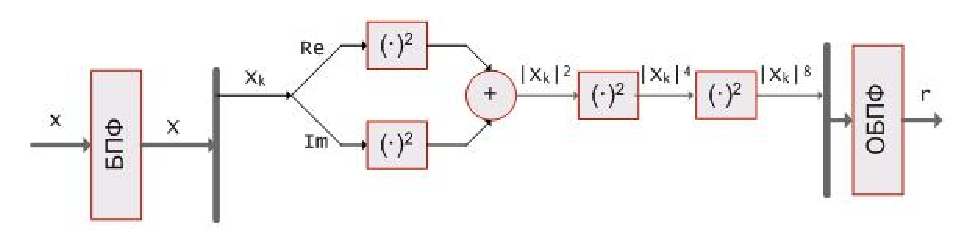
\includegraphics[width=1\linewidth]{akf_fft.eps}}
	\caption{Усовершенствованный итеративный алгоритм получения АКФ}
	\label{pic:akf_pic}
\end{figure}

Количество умножений необходимых для оценки АКФ прямым методом: ${OP_{ACF} = 3N^2}$. Количество умножений необходимых для оценки
усовершенствованным итеративным алгоритмом получения АКФ: ${OP_{ACF\_FFT} = 8NlogN + (k+2)N}$.

ОСШ в оценке АКФ по мощности можно вычислить по известной формуле:
\begin{center}
\begin{equation}
	\label{eq:akf_max_eq}
	R_s=2 B T R_e \frac{1}{2+1/R_e}
\end{equation}
\end{center}
где ${R_s}$ - оченка ОСШ для АКФ, ${R_e}$ - ОСШ исходного сигнала, ${T}$ - длинна выборки (сек), ${B}$ -  ширина спектра сигнала.

На рисунке \ref{pic:gps_spectrum} представлен спектр после повторной
модуляции ПСП. В случае наличия интерференции, представляющей собой окрашенный шум, оценка параметрическим методом даст смещенное значение.
Применение усовершенствованного алгоритма итеративного вычисления АКФ позволяет получить ярко выраженный пик в спектральной области,
а СПМ приобретает симметричный вид, что позволяет использовать АР модель второго порядка для получения несмещенной оценки частоты
широкополосного сигнала.

После трех 
итераций предлагаемого алгоритма спектральный пик существенно вырастает над уровнем шума - рисунок \ref{pic:GPS_spectrum_iter3}.

\begin{figure}[H]
	\center\scalebox{0.8}{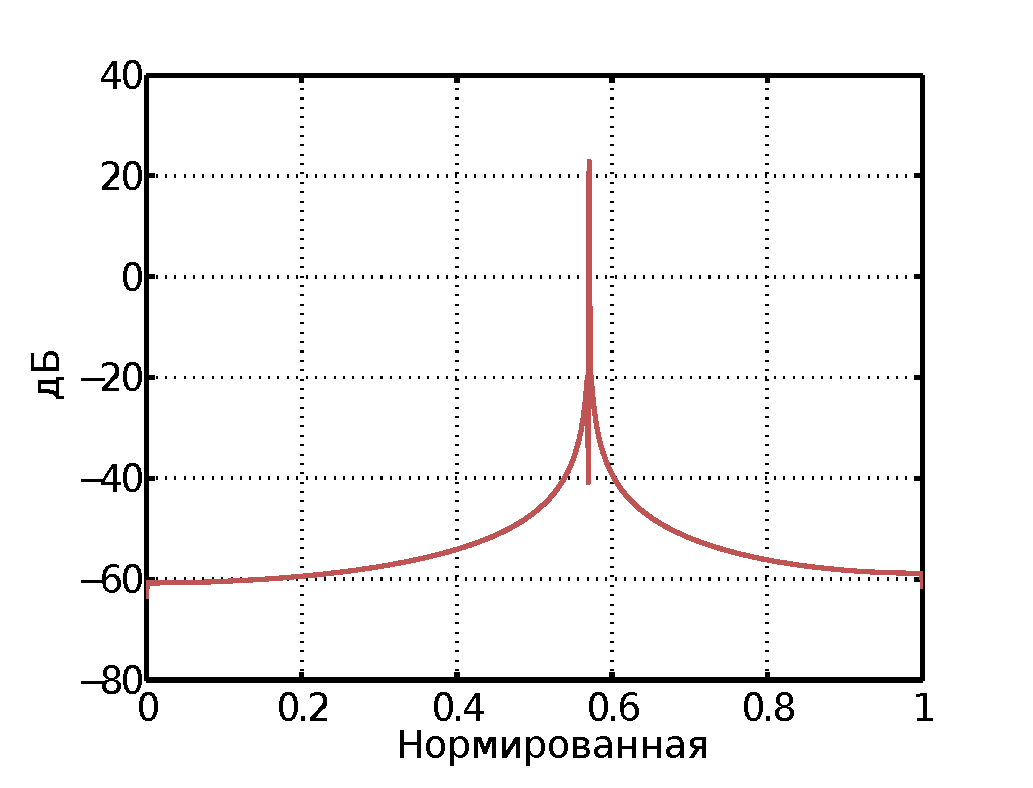
\includegraphics[width=1\linewidth]{GPS_spectra_iter3.eps}}
	\caption{СПМ сигнала после 3 итерации уточнения АКФ}
	\label{pic:GPS_spectrum_iter3}
\end{figure}



\paragraph{В третьей главе} рассматривается параметрический метод оценки частоты на основе авторегрессионной (АР) - модели сигнала.

Удобство применения АР для задачи оценки частоты обусловлено тем, что в сигнале с расширенным спектром после демодуляции ПСП остается одна
гармоническая компонента и шум (\ref{eq:cdma_strip_eq}).  Даже если входной сигнал содержал другие гармонические компоненты,
после повторной модуляции они будут "размазаны" по спектру.

Для обнаружения одного гармонического сигнала на фоне аддитивной помехи в виде белого шума достаточно использовать АР модель второго порядка.

Но на качество оценки параметра сильное значение имеет качетво оценки АКФ. Для оценки, удовлетворяющий ФАПЧ, необходима более точная
оценка АКФ, чем можно получить вычисляя АКФ без предварительно компенсации шума.

Компенсация шума с помощью предлагаемого итеративного алгоритма позволяет достичь заданной точности при уровне ОСШ -25 дБ, в то
время как без компенсации шума заданная точность может быть достигнута только при уровне 10 дБ - рисунок \ref{pic:ACF_boost}.

\begin{figure}[H]
\center\scalebox{1}{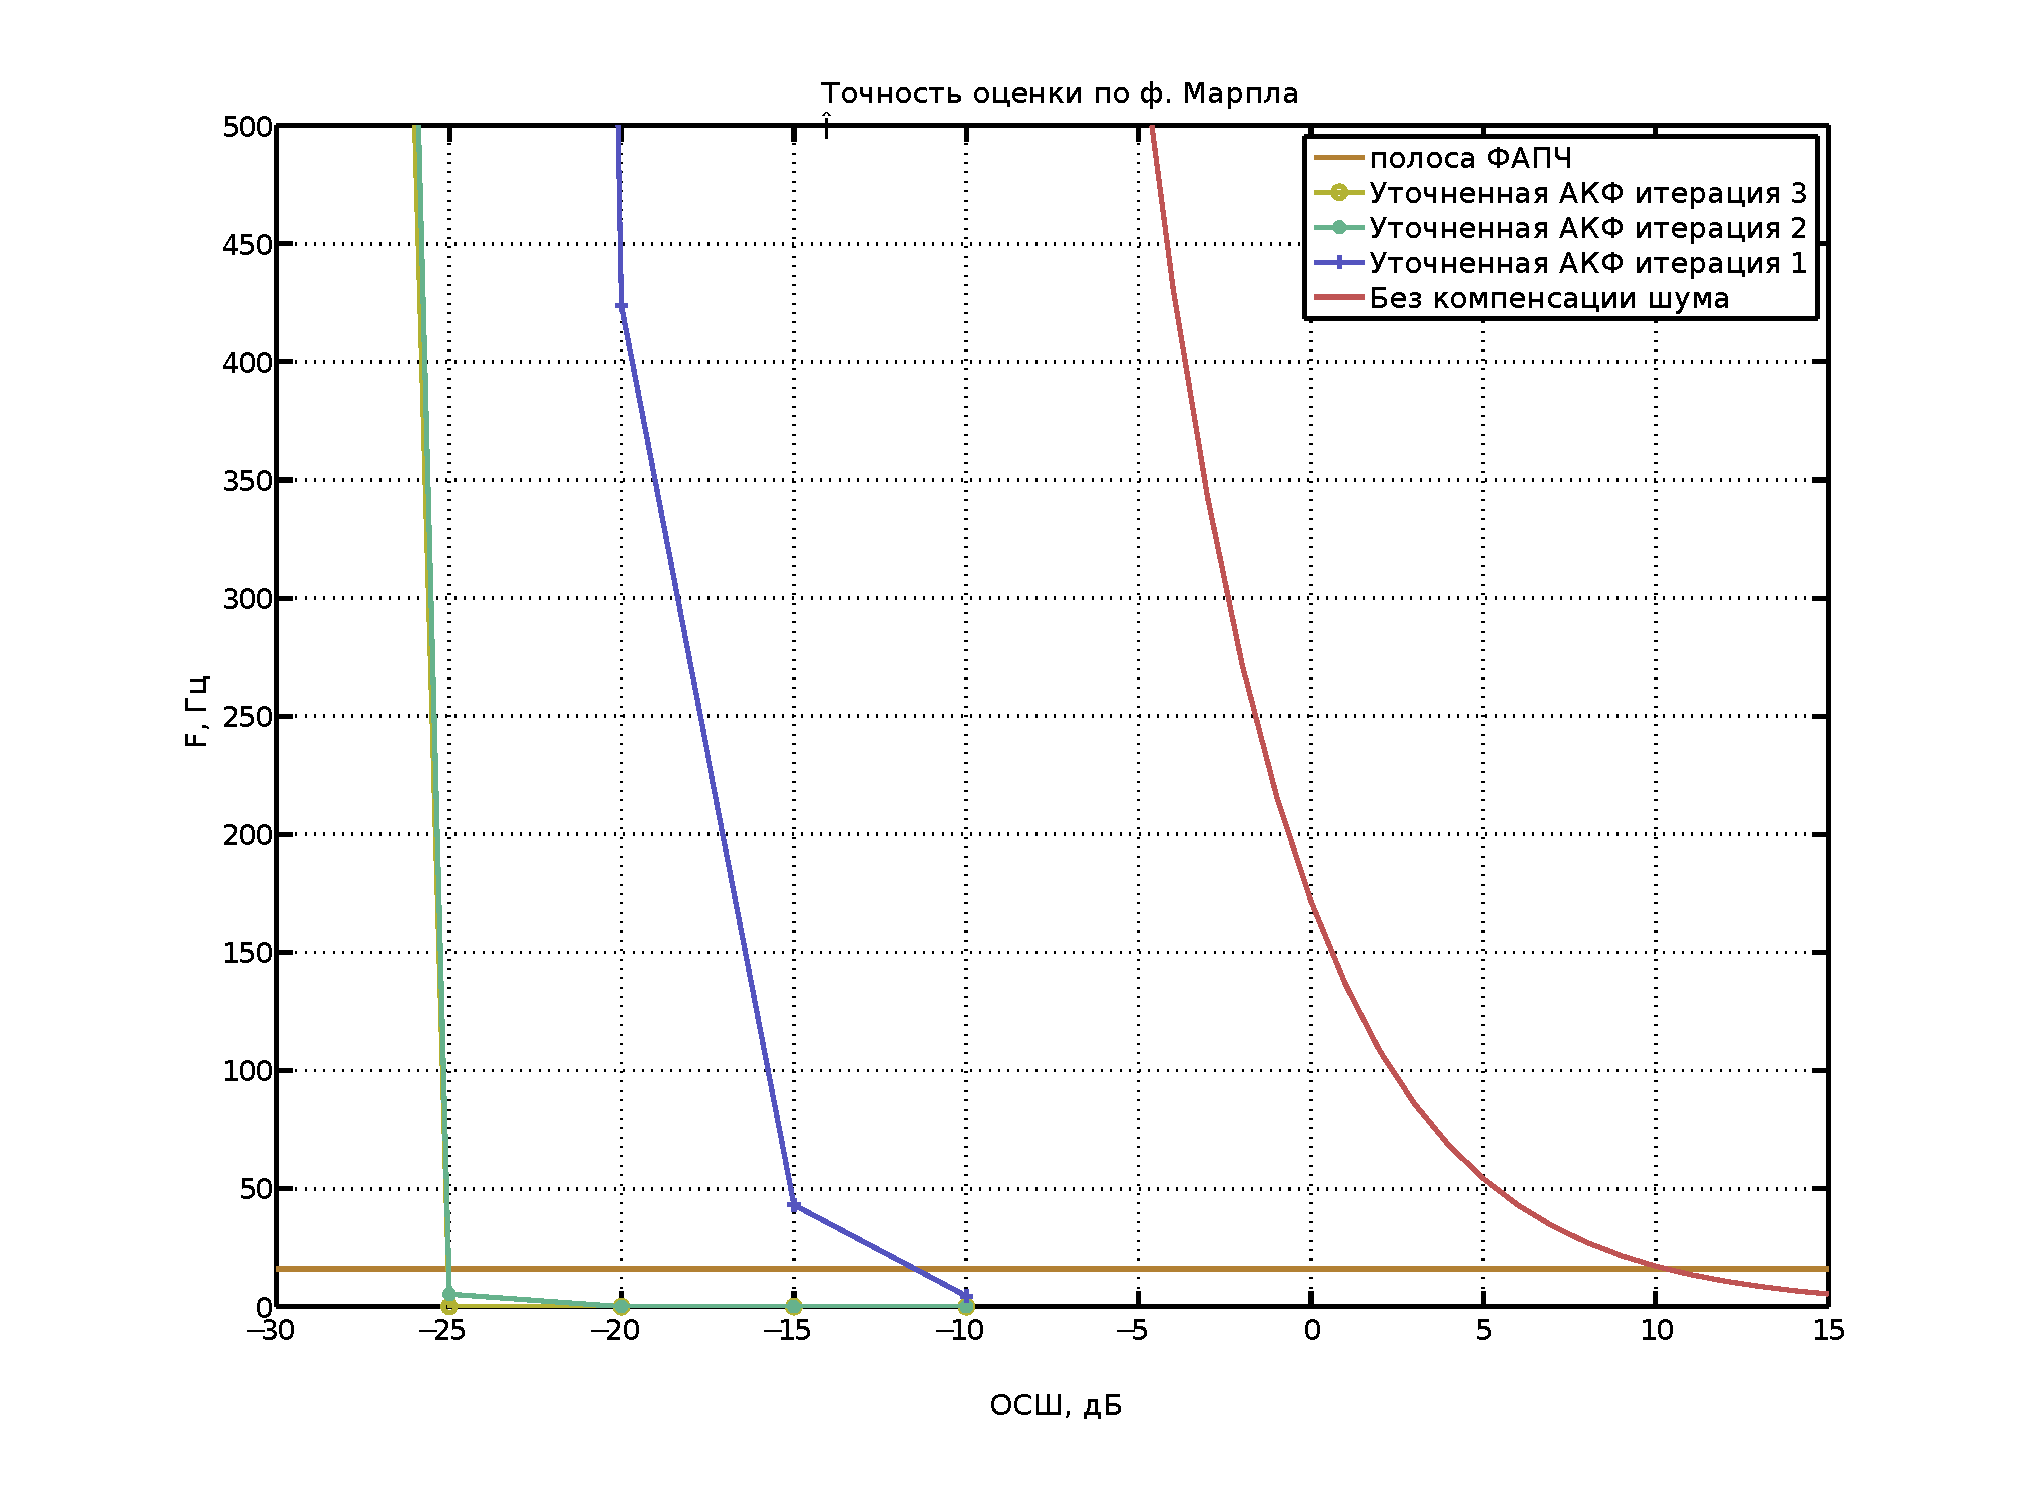
\includegraphics[width=1\linewidth]{ACF_boost.eps}}
	\caption{Точность оценки частоты с компенсацией и без компенсации шума}
	\label{pic:ACF_boost}
\end{figure}

%\paragraph{Оценка частоты с использованием АР-модели}

Для использования АР-модели в задаче оценки частоты сигнала в сетях с широкополосными сигналами, необходимо знать фазу ПСП.
Для оценки фазы ПСП в данной работе используется алгоритм Delay and Multiply Approach, который предложен в \cite{tsui, lin_dma}.
Данный алгоритм позволяет свести перебор в двух областях: частота и фаза ПСП к перебору в одной - фаза ПСП.
Стоит отметить недостаток алгоритма DMA – невозможность использовать в слабых сигналах, так как алгоритм увеличивает уровень шума
в процессе детектирования.

Схематично приемник с использованием АР-модели для оценки частоты представлен на рисунке \ref{pic:ar_cdma_scheme}.
Точность оценки частоты АР-методом позволяет использовать значение оценки непосредственно в качестве начального значения для запуска ФАПЧ.

\begin{figure}[H]
	\center\scalebox{1}{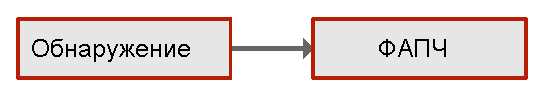
\includegraphics[width=1\linewidth]{ar_scheme.eps}}
	\caption{Схема приемника на основе АР-модели}
	\label{pic:ar_cdma_scheme}
\end{figure}

Разрешающая способность оценки частоты и использованием АР-метода зависит от величины ОСШ. В данной работе рассматривается
АР-модель 2 порядка с одной гармонической компонентой, тем не менее представляется возможным использовать приближенную
формулу Марпла \cite{kay_ar_book, marpl_book} для оценки разрешающей способности:

\begin{equation}
	\label{eq:ar_cdma_marple_eq}
	F = \frac{1.03}{Tp[SNR(p+1)]^{0.31}}
\end{equation}
где ${F}$ – разрешение в герцах, ${Т}$ - интервал отсчетов в секундах, p-максимальное значение временного сдвига для АКФ
последовательности, а ${SNR}$ - ОСШ выраженное в линейных единицах. В задаче оценке частоты в ПСП-модулированном сигнале ${p=2}$.
График зависимости точности от ОСШ представлен на рисунке \ref{pic:cdma_ar_marple_eq}.

\begin{figure}[H]
	\center\scalebox{0.8}{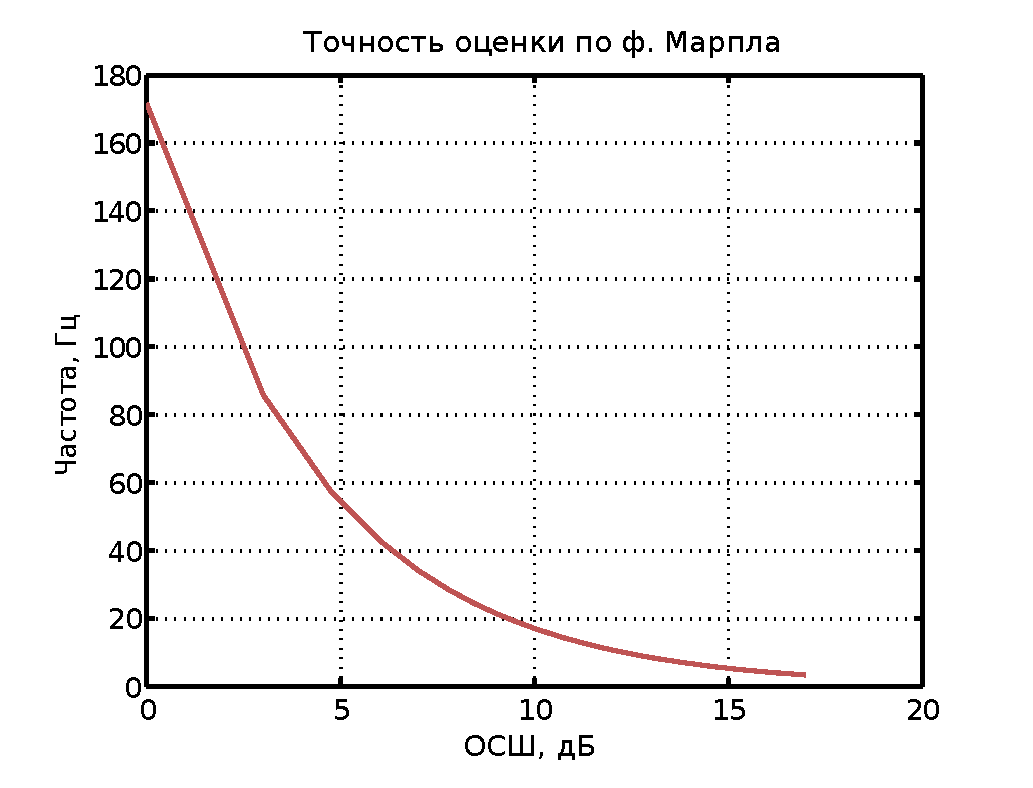
\includegraphics[width=1\linewidth]{marple_eq.eps}}
	\caption{Оценка зависимость точность оценки частоты от ОСШ по ф. Марпла}
	\label{pic:cdma_ar_marple_eq}
\end{figure}

\paragraph{В четвертой} главе приводится имитационное моделирование развиваемых алгоритмов. В качестве алгоритма
для сравнения используется параллельный коррелятор с алгоритмом уточнения частоты.

Алгоритм оценки параметров ШПС в условиях интерференции (Delay and Multiply Approach + уточненный АР).
В работе предлагается объединить результаты работы алгоритма Delay and Multiply Approach и, предложенных
в данной работе, усовершенствованного итеративного алгоритма уточнения АКФ гармонического
сигнала и подхода для оценки частоты широкополосного сигнала при помощи АР-модели.

Схематично приемник изображен на рисунке \ref{pic:ar_dma_scheme}.

\begin{figure}[H]
\center\scalebox{1}{\includegraphics[width=1\linewidth]{dma_quadruple_lpc.eps}}
	\caption{Алгоритм обнаружения и оценки параметров ШПС в условиях интерференции (DMA + уточненный АР)}
	\label{pic:ar_dma_scheme}
\end{figure}

Выходом алгоритма Delay  является оценка фазы ПСП. Повторно модулируя входящий сигнал ПСП с полученной
фазой, можно восстановить гармонический сигнал. Для оценки частоты данного сигнала применяется
АР-метод. Но для оценки АР-методом, требуется точная оценка АКФ, которую можно получить
с помощью усовершенствованного итеративного алгоритма вычисления АКФ.

{\underline{Предложенный алгоритм можно описать следующим набором шагов:}}
\begin{itemize}
\item[Шаг 1.] Входной сигнал ${x(m)}$ умножается на задержанную копию ${x(m-\tau)}$. Так же
	на данном шаге можно производить когерентное накопление результата, для
	увеличения ОСШ.

	\begin{center}
	\begin{equation}
		%\label{}
		x_{new}(m) = \frac{C_{new}(k)}{2} \left(\cos (2\pi f \tau) - \cos \left[2 \pi f (2m - \tau)\right]\right)
	\end{equation}
	\end{center}

\item[Шаг 2.] Полученный сигнал ${x_{new}(m)}$ фильтруется ФНЧ для отсечения высокочастотной компоненты.
\item[Шаг 3.] Генерируется локальная ПСП ${C(m)}$ и умножается на задержанную копию ${C(m-\tau)}$.

	\begin{center}
	\begin{equation}
		%\label{}
		C_{new}(m) = C(m)C(m-\tau)
	\end{equation}
	\end{center}

\item[Шаг 4.] Отфильтрованный сигнал ${x_{filt}(m)}$ коррелируется с новой ПСП ${C_{new}(m)}$
	с использованием БПФ. Выход коррелятора сравнивается с заранее определенным порогом.

	\begin{center}
	\begin{equation}
		%\label{}
		x_{filt}(m) = \frac{C_{new}(m)}{2} \cos (2\pi f \tau)
	\end{equation}
	\end{center}

	\subitem{\underline{Если}}  значение оказалось больше порогового {\underline{то}},
		принимается решение о наличии сигнала. Полученное значение фазы ПСП  - ${k}$ запоминается.
		Перейти на шаг 5.
	\subitem{\underline{Иначе}} 
		Выбирается ${N}$ максимальных значений и запоминаются их фазы ПСП.
\item[Шаг 5.] Входной сигнал ${x(m)}$ модулируется ПСП ${C(m-k)}$, где ${k}$ - это фаза ПСП из ${N}$ - выбранных. В результате получаем гармонический
	сигнал ${x_{cos}(m)}$ с неизвестной частотой.
\item[Шаг 6.] Для увеличения ОСШ сигнала ${x_{cos}(m)}$ вычисляется значение уточненное значение АКФ
	по усовершенствованному итеративному алгоритму получения АКФ.
\item[Шаг 7.] Определяются коэффициенты АР-модели ${\hat{a_1}, \hat{a_2}}$.
	Вычисляется резонансная частота ${\omega_1}$ и определяется квадрат модуля частотного отклика АР-модели для этой частоты. 
\item[Шаг 8.]
	Сравнение квадрата модуля с порогом.
        \subitem{\underline{Если}}  значение оказалось больше порогового {\underline{то}} 
                принимается решение о наличии сигнала, а в качестве оценки
                частоты принимается значение ${\omega_1}$ соответствующее выбранной фазе ПСП. 
        \subitem{\underline{Иначе}} 
		\subsubitem\underline{Если} остались непроверенные фазы ПСП - переход на шаг 5.
		\subsubitem\underline{Иначе} сигнал не обнаружен.
\end{itemize}

Общее количество умножений, необходимых для детектирования и оценки частоты от одного источника предлагемым
алгоримом (количество итераций в алгоритме уточнения АКФ ${k=3}$): ${OP_{DMA\_ACF\_AR} = 16NlogN + 11N + 51}$.

Количество итераций требуемых для оценки частоты одного источника параллельным корррелятором:
${OP_{corr} = 48NlogN + 65N}$.

График вероятности оценки частоты в допустимом даипазоне входной расстройки представлен на рисунке
\ref{pic:ar_dma_probability}. Моделирование проводилось с аддитивным шумом, заданным в полосе от 0 Гц до
половины частоты дискретизации для одного, двух и трех шагов уточнения АКФ.

\begin{figure}[H]
\center\scalebox{1}{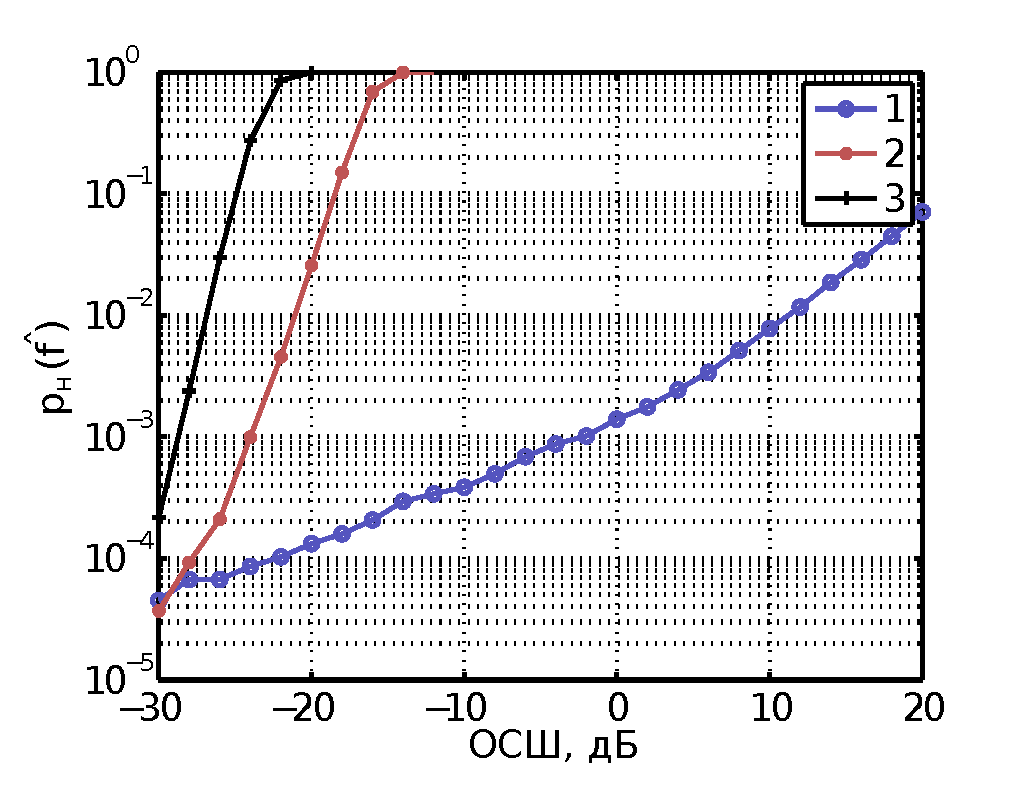
\includegraphics[width=1\linewidth]{ar_dma_probability.eps}}
	\caption{Ве}
	\label{pic:ar_dma_probability}
\end{figure}

Предлагаемый подход существенно выигрывает по вычислительным затратам в сравнении с параллельным коррелятором.



\paragraph{Применение АР-метода для детектирования сигнала с расширенным спектром}

Рассмотрим применение данного подхода для детектирования одного сигнала ШПС на фоне аддитивного белого шума.
Схема алгоритма представлена на рисунке \ref{pic:ar_cdma1_scheme1}.

\begin{figure}[H]
	\center\scalebox{0.9}{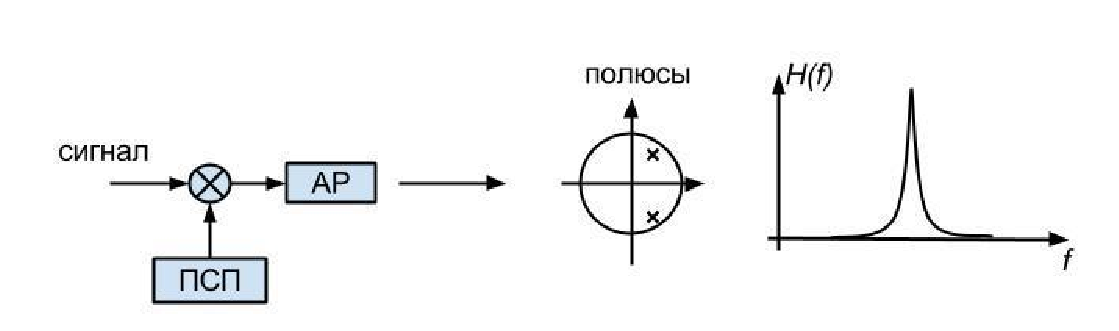
\includegraphics[width=1\linewidth]{lpc_for_1_sat_scheme.eps}}
	\caption{Детектирование сигнала АР-методом при известной фазе ПСП.}
	\label{pic:ar_cdma1_scheme1}
\end{figure}

Для восстановления гармонического сигнала из ШПС входная последовательность умножается на локально сформированную ПСП.
Далее запускается алгоритм на основе АР-модели. В реальных условиях приемник не имеет информации о фазе ПСП поэтому для детектирования
сигнала необходимо перебрать все возможные смещения расширяющего кода. Для ускорения вычислений предлагается использование алгоритма быстрого преобразования Фурье (БПФ).
Схема вычислений представлена на рисунке \ref{pic:ar_cdma1_scheme2}.

\begin{figure}[H]
	\center\scalebox{0.9}{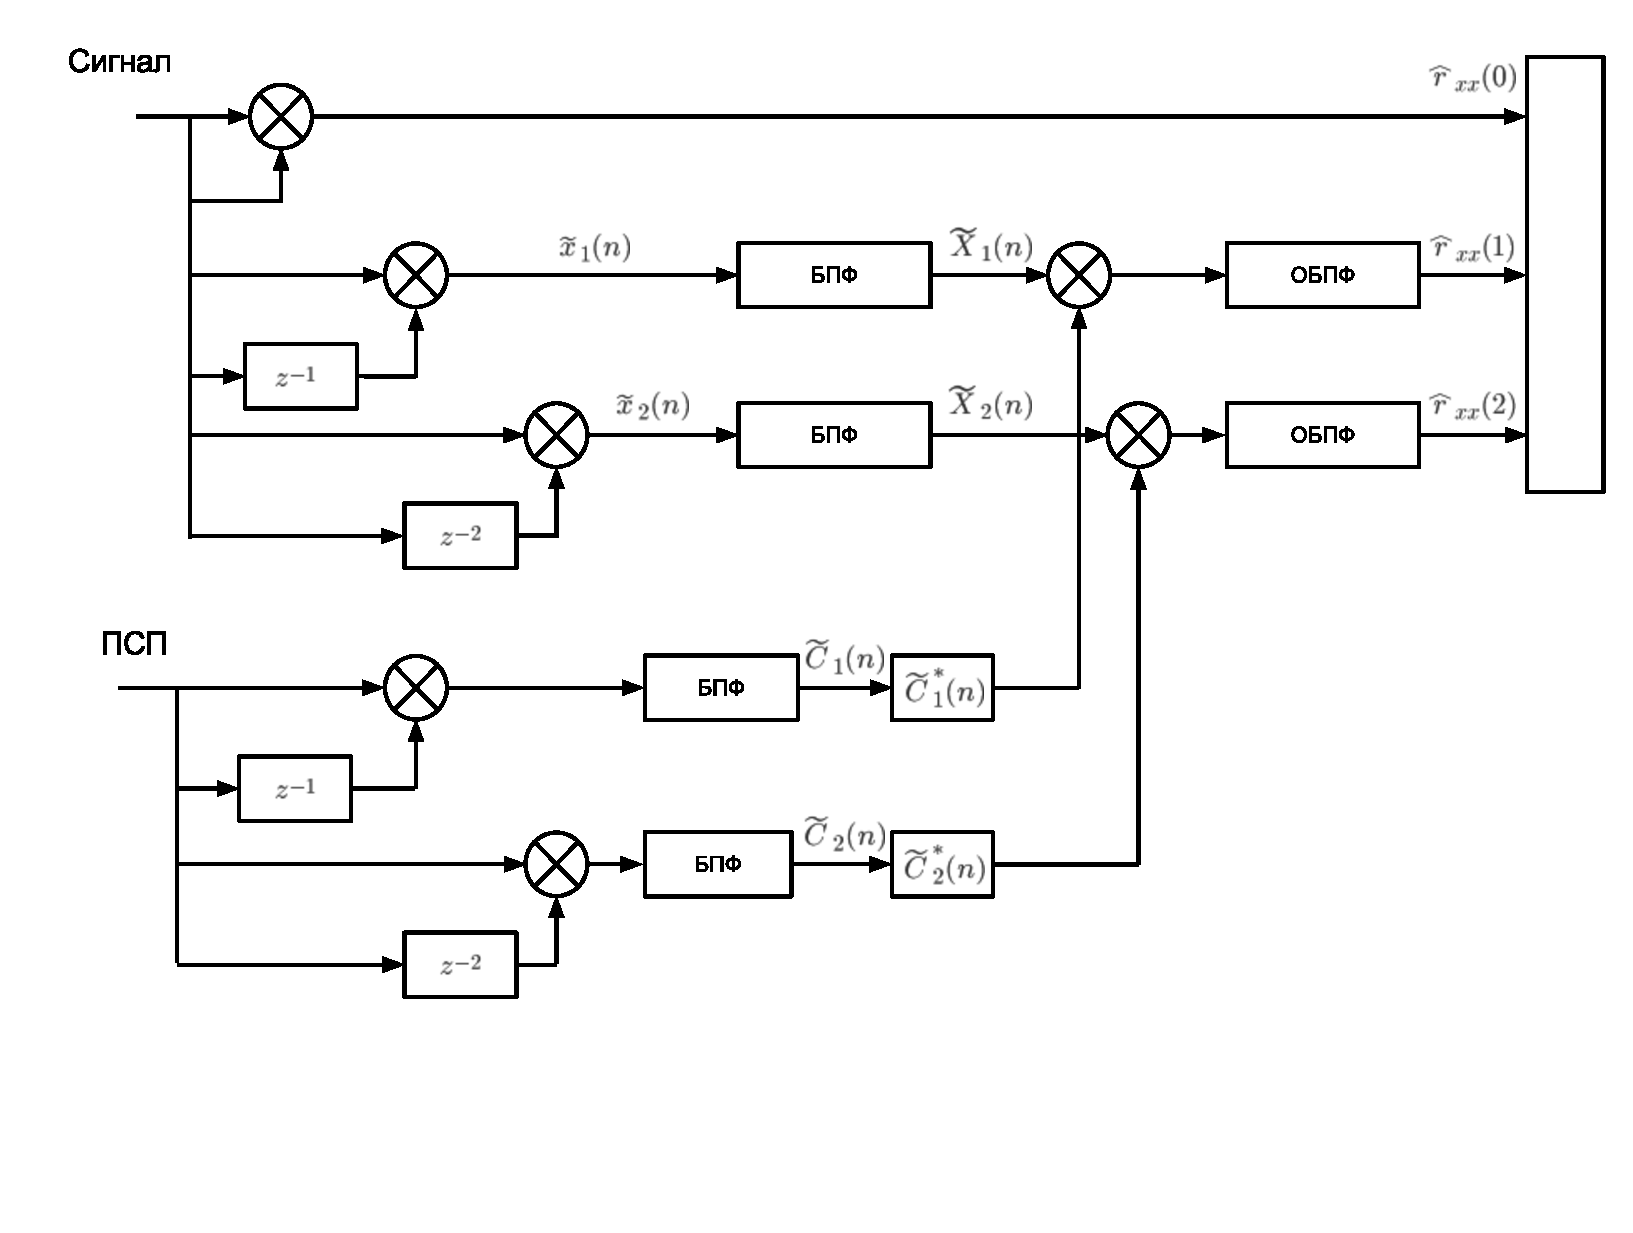
\includegraphics[width=1\linewidth]{lpc_fft.eps}}
	\caption{Общая схема применения АР модели для детектирования ШПС сигнала.}
	\label{pic:ar_cdma1_scheme2}
\end{figure}

Оценка ${\hat{r}_{xx}(0)}$ не зависит от выбранной фазы ПСП, поэтому она вычисляется один
раз для всех смещений кода. Далее формируется массив произведений входного сигнала на
свою задержанную копию ${\tilde{x}_1(n)=x(n)x(n-1)}$. Полученная последовательность  
${\tilde{x}_1(n)}$ поступает на вход алгоритма БПФ, в результате получаем массив ${\tilde{X}_1(n)}$
содержащий частотные отсчеты. Аналогично формируется массив  ${\tilde{X}_2(n)}$ для
задержки входного сигнала равной двум. Таким же способом обрабатываются локально
сгенерированные ПСП и формируются два массива ${\tilde{C}_1(n)}$ и ${\tilde{C}_2(n)}$.
Далее массивы ${\tilde{X}_1(n)}$ и ${\tilde{X}_1(n)}$ поэлементно перемножаются
на комплексно сопряженные массивы ${\tilde{C}_1^*(n)}$ и ${\tilde{C}_2^*(n)}$.
Результаты этих перемножений поступают на вход алгоритма обратного
БПФ. Полученные после ОБПФ два массива содержат оценки автокорреляционной функции для ${N}$ 
смещений кода, где  ${N}$ - размер данных на входе алгоритма БПФ.

Таким образом, предлагаемый алгоритм состоит из следующих шагов:

\begin{itemize}
\item[Шаг 1.] Вычисляются оценки  АКФ в трех первых точках (для аргументов АКФ=0,1,2)
	с использованием алгоритма БПФ для всех возможных смещений ПСП. 
\item[Шаг 2.] Для каждого смещения ПСП: 
	Определяются коэффициенты АР-модели ${\hat{a_1}, \hat{a_2}}$, 
	по формуле \ref{eq:ar_coef_matrix}.
	Вычисляется резонансная частота ${\omega_0}$
	и определяется квадрат модуля частотного отклика АР-модели для этой частоты. 
\item[Шаг 3.] Выбирается смещение ПСП для которого значение квадрата модуля частотного отклика было максимальным. Полученное значение сравнивается с заранее выбранным порогом детектора. 
	\subitem{\bf{Если}}  значение оказалось больше порогового {\bf{то}} 
		принимается решение о наличии сигнала, а в качестве оценки
		частоты принимается значение ${\omega_0}$ соответствующее выбранному смещению ПСП. 
	\subitem{\bf{Иначе}} 
		Принимается решение об отсутствии гармонического сигнала.
\end{itemize}

Разработанный алгоритм позволяет производить оценку частоты гармонического сигнала без использования прямого перебора как это делается в большинстве современных алгоритмов.
Например, алгоритм Delay and Multiply Approach (DMA) предложенный в \cite{tsui,lin_dma} позволяет производить поиск только по смещению ПСП,
но он не дает возможности прямой оценки частоты. Для оценки частоты и принятия решения о наличии сигнала в алгоритме DMA необходимо использовать стандартный коррелятор.
Предложенный алгоритм допускает сокращение количества операций умножения при переборе значений фазы ПСП за счет использования алгоритма БПФ.

\begin{figure}[H]
	\center\scalebox{1}{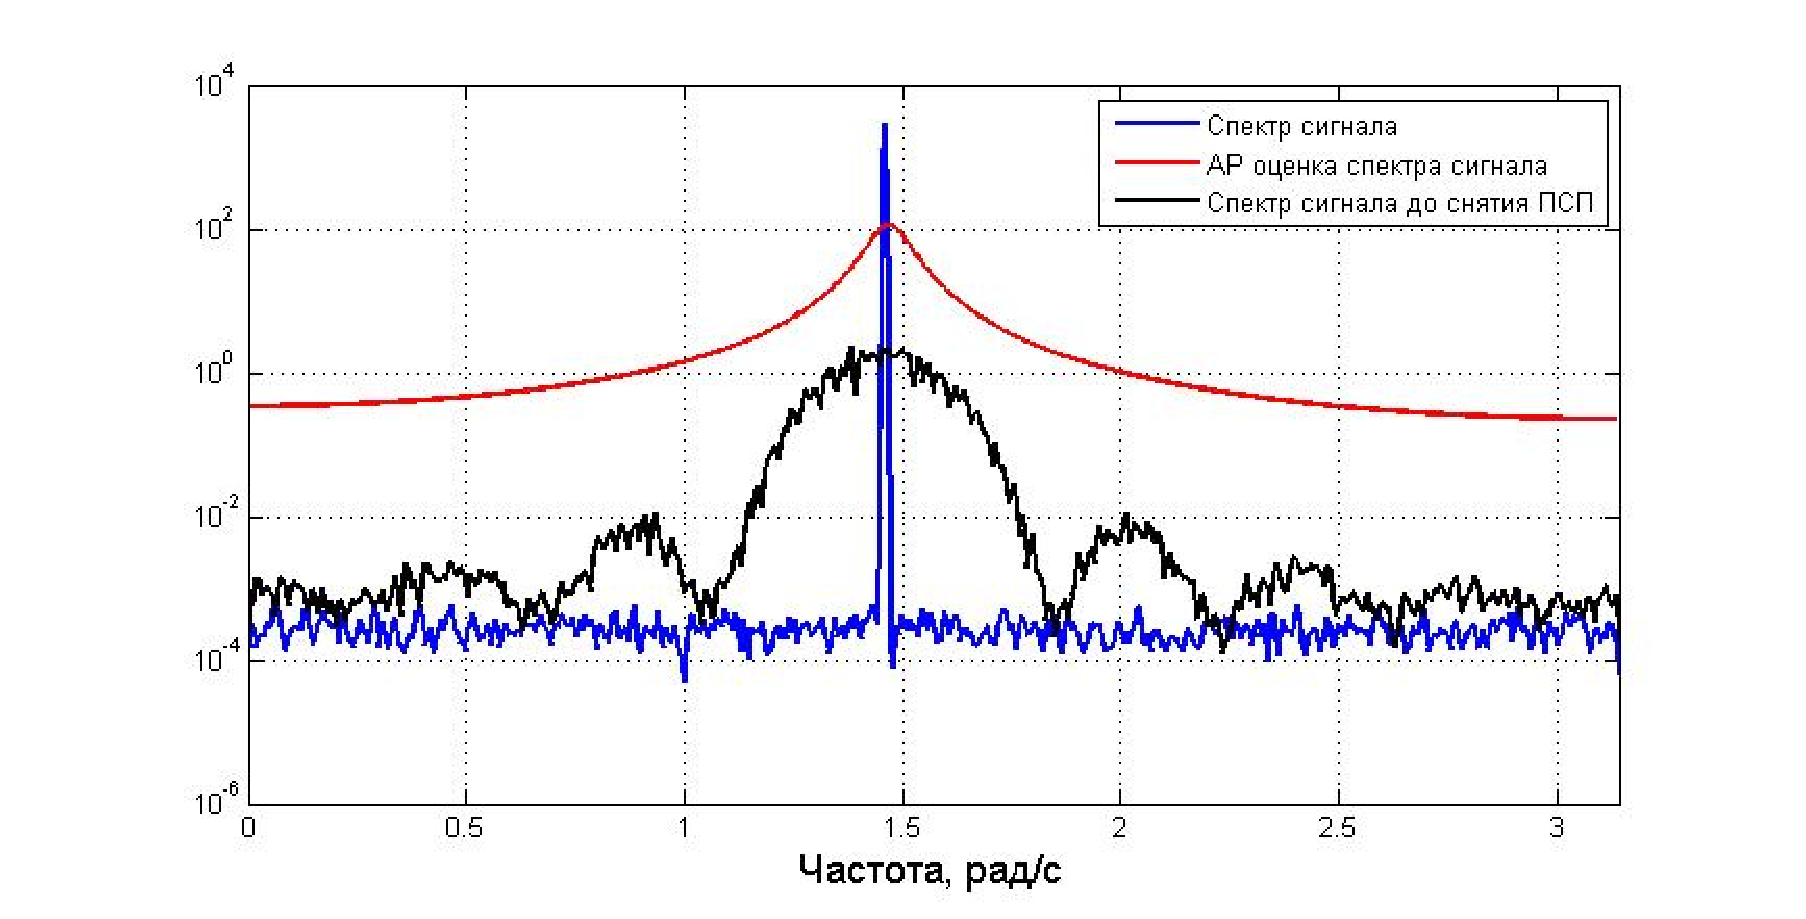
\includegraphics[width=1\linewidth]{lpc_1sat.eps}}
	\caption{Оценка СПМ сигнала модулированного ПСП}
	\label{pic:ar_cdma1_freq_est1}
\end{figure}

Основным недостатком предложенного алгоритма является сильная чувствительность по отношению к интерференционным помехам: наличие «окрашенного» шума приводит к
значительному смещению получаемых оценок частоты и мощности гармонического сигнала - рисунок \ref{pic:ar_cdma1_freq_est2}.

\begin{figure}[H]
	\center\scalebox{1}{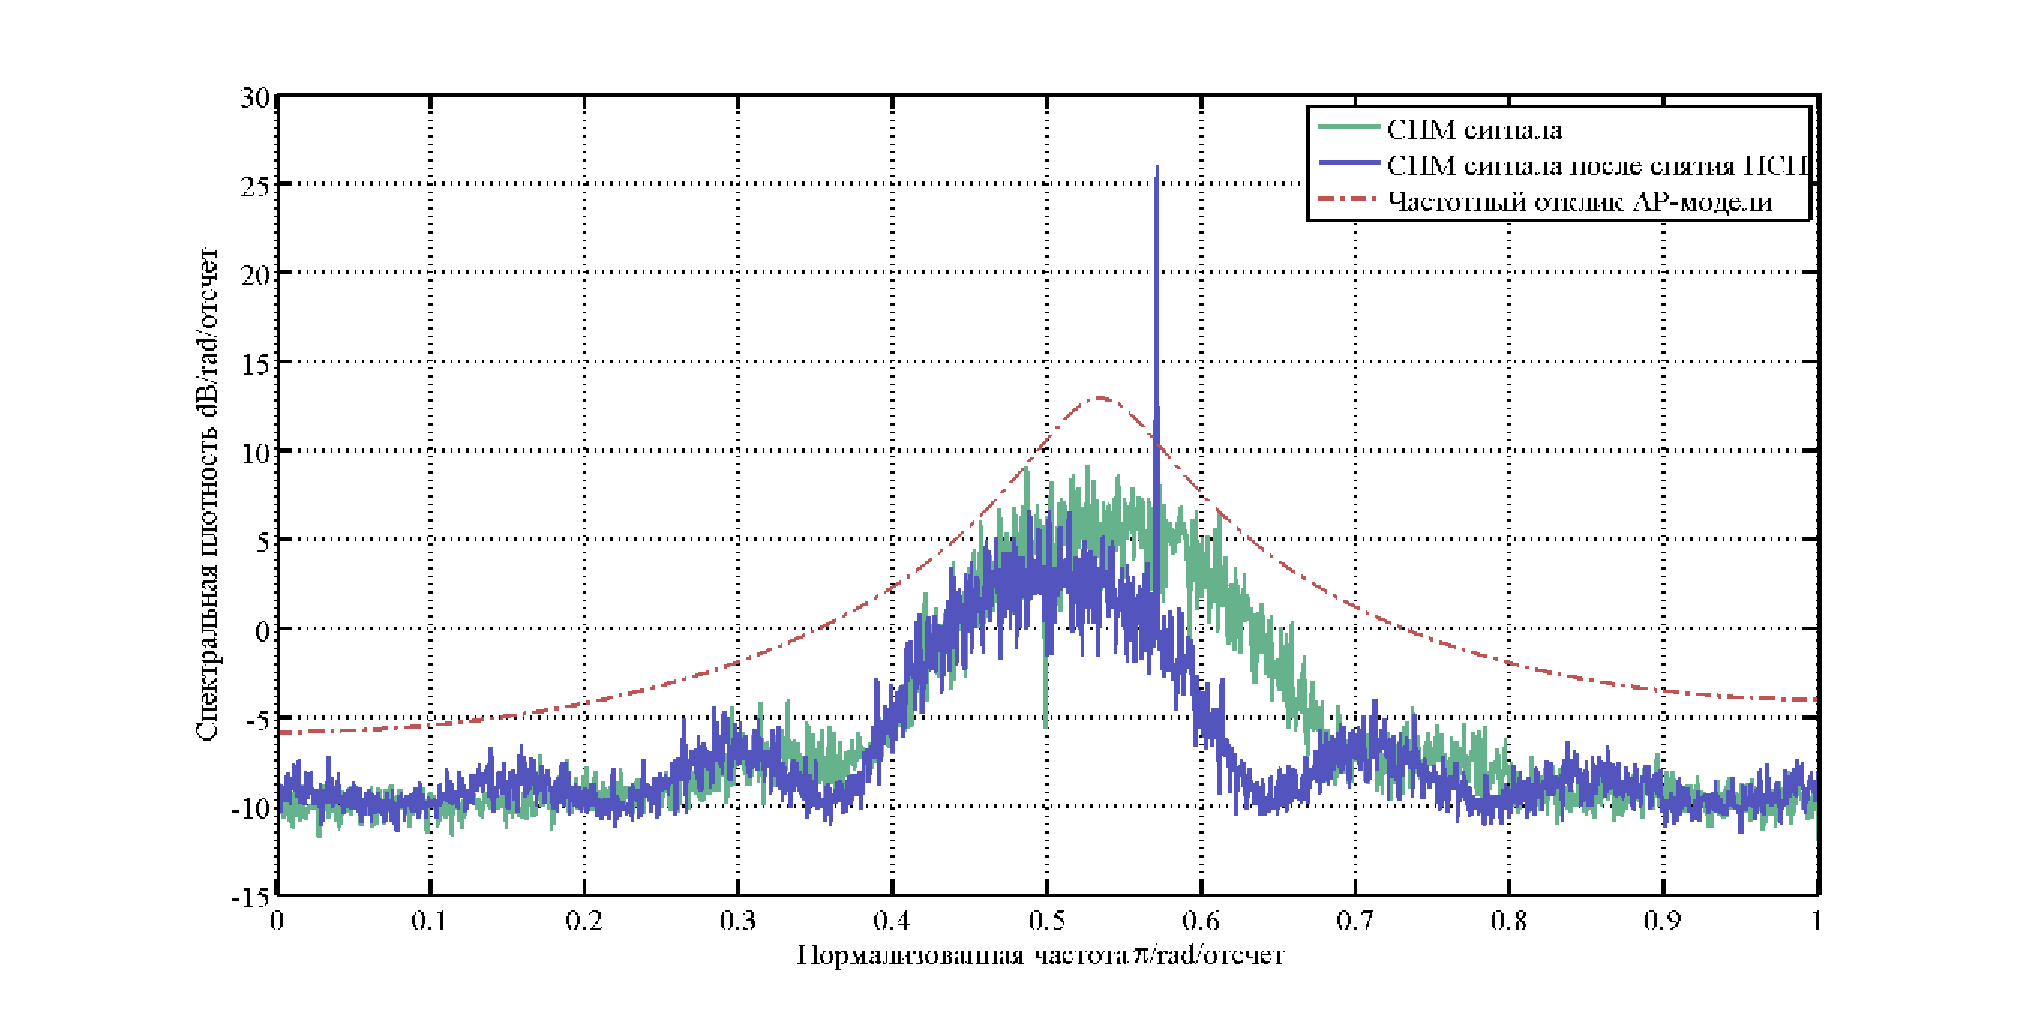
\includegraphics[width=1\linewidth]{lpc_2sat_psd.eps}}
	\caption{Оценка сигнала модулированного ПСП при наличии интерференции}
	\label{pic:ar_cdma1_freq_est2}
\end{figure}


{\bf{В заключении}}
отражены результаты работы и обозначены направления дальнейшего исследования

\noindent\centerline{\bf{Основные результаты и выводы}}
В ходе диссертационного исследования получены следующие результаты:
\begin{enumerate}
\item Разработан алгоритм на основе параметрического метода оценки частоты для одного источника с широкополосным сигналом.
\item Усовершенствован алгоритм итеративного вычисления автокорреляционной функции, что позволяет использовать его в приемниках
	реального времени.
\item Разработан алгоритм оценки параметров широкополосного сигнала на основе алгоритма Delay and Multiply Approach с использованием
	предложенного усовершенствованного итеративного алгоритма вычисления автокорреляционной функции и параметрического
	метода оценки частоты. Данное решение имеет более высокую точность оценки в сравнении с традиционным
	параллельным коррелятором, в то же время оценка параметра может быть получена за меньшее количество итераций.
\item Произведено имитационное моделирование предложенного алгоритма для проверки положений, выносимых на защиту.
\item Произведено обоснование актуальности и возможности применения параметрического метода оценки частоты для сигналов
	с расширенным спектром.
\item Отражены возможные направления дальнейших исследований в области применения параметрического анализа в системах
	с расширенным спектром.
\end{enumerate}


\newpage
